\documentclass[a4paper, 12pt, titlepage]{article}
%=======Unpackage Things===============
\usepackage{color}
\usepackage{colortbl}
\usepackage{mathrsfs}

\usepackage{graphicx}
\usepackage{amsthm}
\usepackage{listings}
%\usepackage{fullpage}
\usepackage{epsfig}
\usepackage{amsmath}
\usepackage{latexsym}
\usepackage{amssymb}
\usepackage{amstext}
\usepackage{array}
\usepackage{titlesec}
\usepackage{float}

\titleformat{\section}
    {\normalfont\fontsize{12}{15}\bfseries}{\thesection}
    {1em}{}

%\titleformat{\subsection}
%    {\normalfont\fontsize{5}{5}\bfseries}{\thesection}
%    {1em}{}
\newcommand{\PreserveBackslash}[1]{\let\temp=\\#1\let\\=\temp}
\newcolumntype{C}[1]{>{\PreserveBackslash\centering}p{#1}}
\newcolumntype{R}[1]{>{\PreserveBackslash\raggedleft}p{#1}}
\newcolumntype{L}[1]{>{\PreserveBackslash\raggedright}p{#1}}


\begin{document}
%==title==
\title{COMP6321 Assignment 3}
\setcounter{tocdepth}{2}
\newpage
\begin{center}
    {\huge COMP6321: Assignment \#3}


    \vspace{2cm}
    Student: Qing Gu  \hspace{5cm}
    Student ID: 6935451
    \vspace{1cm}

    =================================================
\end{center}
\section{A Midterm Preparation Question}
\section{Properties of Entropy}
\subsection{Evaluating Entropies}
According to the given joint probability, we can come out with the following probability:
$$p\{x=1\} = \frac{1}{3}; p\{x=0\} = \frac{2}{3}$$
$$p\{y=1\} = \frac{2}{3}; p\{y=0\} = \frac{1}{3}$$
According to the entropy euqations:
$$ H[x] = \Sigma_{i=1}^np(x_i)I(x_i)=-\Sigma_{i=1}^np(x_i)\log{p(x_i)}$$
$$ H[Y|X] = \Sigma_{x\in{}X, y\in{}Y}p(x,y)\log{\frac{p(x)}{p(x,y)}}$$
$$H[Y|X]=H[X,Y]-H[X]$$
$$I[X,Y] = \Sigma_{y\in{}Y, x\in{}X}p(x,y)\log{\frac{p(x,y)}{p(x)p(y)}}$$
The following entropies and information can be calculated
\begin{itemize}
    \item $H[x] = -(\frac{1}{3}\log{\frac{1}{3}}+\frac{2}{3}\log{\frac{2}{3}})=\log{3}-\frac{2}{3}\log{2}$
    \item $H[y] = -(\frac{1}{3}\log{\frac{1}{3}}+\frac{2}{3}\log{\frac{2}{3}})=\log{3}-\frac{2}{3}\log{2}$
    \item $H[y|x] = \frac{2}{3}\log{\frac{2/3}{1/3}}+\frac{1}{3}\log{\frac{1/3}{1/3}}=\frac{2}{3}\log{2}$
    \item $H[x|y] = \frac{2}{3}\log{2}$
    \item $H[x,y] = H[y|x] + H[x] = \log{3}$
    \item $I[x,y] = H(x) - H(x|y) = \log{3} - \frac{4}{3}\log{2}$
\end{itemize}
\subsection{Maximum Entropy Discrete Distribution}
For discrete distribution, the maximum problem can be interpreted like this:
$$\max{}\Sigma{}p_i\log{1/p_i}$$
$$w.r.t~\Sigma{}p_i=1$$
Form the Lagrangian:
$$L(P, \lambda) = \Sigma{}p_i\log{1/p_i} + \lambda{\Sigma{}p_i-1}$$
Let $\frac{\delta}{\delta\lambda}L=0$ we get $\Sigma{}P_i=1$. This is the original constraint which is irrelevant with $\lambda$.

Let $\frac{\delta}{\delta{}p_j}L=0$ (Probability of an arbitrary event), we get $p_j = 2^{\lambda-1}$. Thus, entropy reaches its maximum the probability when every event is equal to a same constant. So the maximum entropy of a discrete probability is achieved for a uniform distribution.

\subsection{Proof of T1}
\begin{center}

    \small

    \centering

    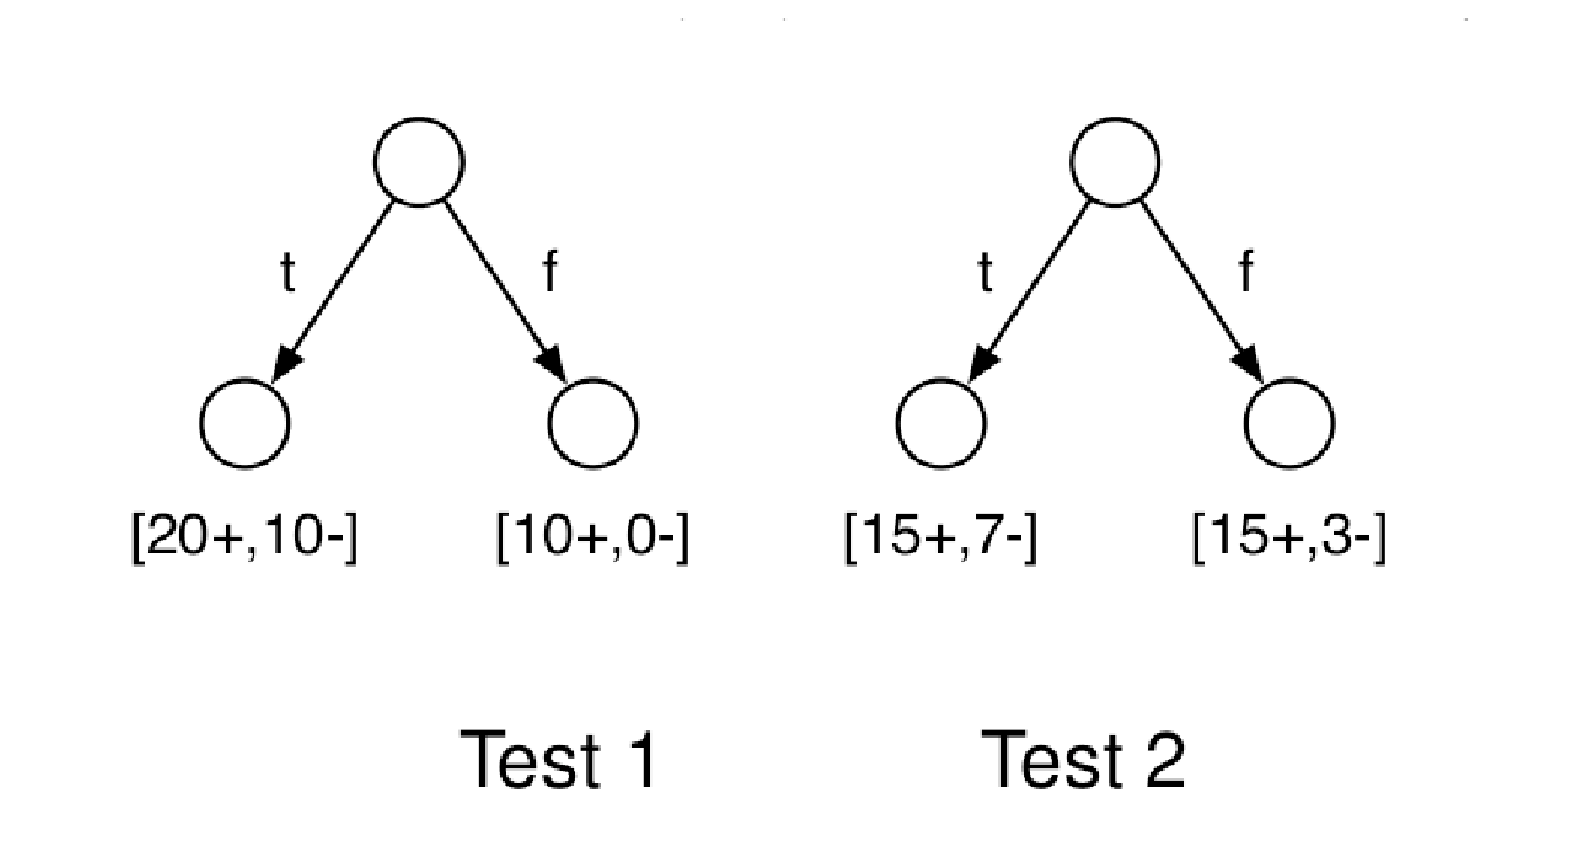
\includegraphics[width=12cm]{tests.eps}

    %\figcaption{UML}

    \label{uml}

\end{center} 
In order to prove T1 is better than T2, we have to prove that Test 1 gained more information. $IG(D|Test1)$ and $IG(D|Test2)$ are computed separately.
        $$H(D) = \frac{3}{4}\log{\frac{4}{3}}+\frac{1}{4}\log{4}=2-\frac{3}{4}\log{3}~bit$$
\begin{itemize}
        \item Information Gain of Test 1
            $$H(D|Test1) = \frac{3}{4}(\frac{2}{3}\log{\frac{3}{2}} + \frac{1}{3}\log{3}) \approx 0.689$$
            $$IG(D,Test1) = H(D) - H(D|Test) \approx 0.123$$
        \item Information Gain of Test 2
            $$H(D|Test2) = \frac{22}{40}(\frac{15}{22}\log{\frac{22}{15}} + \frac{7}{22}\log{\frac{22}{7}}) + \frac{18}{40}(\frac{15}{18}\log{\frac{18}{15}} + \frac{3}{18}\log{\frac{18}{3}})\approx 0.653$$
\end{itemize}:q

\section{Kernels}
\begin{enumerate}
    \item $K(x,z) = aK_1(x,z) + bK_2(X,z)~ a,b>0$

        Using Merceris Theorem:

        Since $K_1$, $K_2$ are kernels, $K_{1ij} = K_{1ji}$, $K_{2ij} = K_{2ji}$. Both kernel matrices are positive semidefinite.
        $$K_{ij} = aK_{1ij} + bK_{2ij} = aK_{1ji} + bK_{2ji} = K_{ji}$$ It's symmetric.
        $$xKx^T = x(aK_1+bK_2)x^T=xaK_1x^T + xbK_2x^T$$
        Since $a,b>0$, K is positive semidefinite.
        Thus, this function is a kernel.
        
    \item $K(x,z) = aK_1(x,z) - bK_2(X,z)~ a,b>0$

        Using Merceris Theorem:

        Since $K_1$, $K_2$ are kernels, $K_{1ij} = K_{1ji}$, $K_{2ij} = K_{2ji}$. Both kernel matrices are positive semidefinite.
        $$K_{ij} = aK_{1ij} - bK_{2ij} = aK_{1ji} - bK_{2ji} = K_{ji}$$ It's symmetric.
        $$xKx^T = x(aK_1-bK_2)x^T=xaK_1x^T - xbK_2x^T$$
        Though $a,b>0$, the relationship of $xaK_1x^T$ and $xbK_2x^T$ can not be determined. $K$ is not a positive semidefinite matrix. Thus, this function is not a kernel.

    \item $K(x,z) = $
\end{enumerate}

\section{Nearest Neighbors vs. Decision Trees}




\end{document}
